% Copyright (C) 2008 Dominik Dahlem <Dominik.Dahlem@cs.tcd.ie>
%
% This file is free software; as a special exception the author gives
% unlimited permission to copy and/or distribute it, with or without
% modifications, as long as this notice is preserved.
%
% This program is distributed in the hope that it will be useful, but
% WITHOUT ANY WARRANTY, to the extent permitted by law; without even
% the implied warranty of MERCHANTABILITY or FITNESS FOR A PARTICULAR
% PURPOSE.

\documentclass[12pt,a4paper]{report}
\usepackage{fancyhdr}
\usepackage[T1]{fontenc}
\usepackage[latin1]{inputenc}
\usepackage{graphicx}
\usepackage{hyperref}
\usepackage{listings}
\usepackage{prettyref}
\usepackage{psfrag}
\usepackage{subfigure}

\def\ccode#1{
  \lstinline[basicstyle=\ttfamily,language=C]{#1} }

\pagestyle{fancy}
\setlength{\headheight}{15pt}

\newrefformat{fig}{\hyperref[{#1}]{Figure~\ref*{#1}}}
\newrefformat{cha}{\hyperref[{#1}]{Chapter~\ref*{#1}}}
\newrefformat{lst}{\hyperref[{#1}]{Listing~\ref*{#1}}}
\newrefformat{sec}{\hyperref[{#1}]{Section~\ref*{#1}}}
\newrefformat{sub}{\hyperref[{#1}]{Section~\ref*{#1}}}
\newrefformat{eq}{\hyperref[{#1}]{Equation~\ref*{#1}}}

\author{Dominik Dahlem}
\title{HPC 563: Classical Simulation}
\date{\today}

\begin{document}
\maketitle

\chapter{Setup}
\label{cha:setup}

\section{General Approach}
\label{sec:general-approach}
\begin{itemize}
\item GNU autotools is used to maintain this project:\\
  autoconf version 2.61 automake version 1.10
\item Getopt is used to parse command-line parameters.\\
  A help message can be displayed by specifying "-?" or "-h" to the
  command-line of the executable.
\item The GSL library was chosen to provide some mathematical
  functions (i.e., \ccode{GSL_MAX} and \ccode{GSL_MIN}) and to control
  the floating point environment of the application.
\item The cunit library was used to implement the unit tests.
\end{itemize}

\section{Configuration}
\label{sec:configuration}
Each feature of the application is configurable. That means that the
libraries required for certain features are checked when the configure
script is executed and an appropriate message is presented to the
user. Some features, such as MPI, GSL, and unit tests have
inter-dependencies which are enforced.

\begin{itemize}
\item The assignment ships with a configure script generated by
  autotools. The following options are supported:
  \begin{itemize}
  \item --enable-test : enables testing using cunit. The unit tests
    require GSL to be configured as well. An error message is
    produced, if the GSL library is not configured or not available.
  \item --enable-gcov : enables the coverage analysis using gcov and
    lcov.
  \item --enable-gsl : enables the GSL library.
  \item --enable-mpi : enables the parallel execution of the
    application using MPI. If MPI is enabled the unit tests are
    disabled, because the tests cannot be executed in a parallel fashion.
  \item --enable-debug : enables debug messages and asserts in some of
    the functions.
  \item --enable-report : Enable the report generation which is
    written in latex.
  \item --enable-plot : Enable the plot generation
  \end{itemize}
\end{itemize}

\section{Make}
\label{sec:make}

The project is set up in such a way that all sources can be built with
a single make command in the root project directory. Additionally, it
is also possible to cd into a c module or the report directory to
build those individually.

\begin{itemize}
\item Installing the application was not considered.
\item To build the project with MPI support do:
  \begin{enumerate}
  \item No gcov, no tests, no MPI
\begin{verbatim}
./configure
make
\end{verbatim}
    Compile the sources
  \item No gcov, no tests, MPI enabled
\begin{verbatim}
./configure --enable-mpi
make
\end{verbatim}
    Compile the sources for parallel execution
  \item No gcov
\begin{verbatim}
./configure --enable-test
make check
\end{verbatim}
    This command will compile everything and run the cunit tests.
  \item Enable gcov and testing
\begin{verbatim}
./configure --enable-test --enable-gcov
make lcov
\end{verbatim}
    This command will compile everything, run the cunit tests, and
    generate a snazzy HTML coverage report using lcov
    \footnote{http://ltp.sourceforge.net/coverage/lcov.php}.
  \item Enable the report generation
\begin{verbatim}
./configure --enable-report --enable-plot
make
\end{verbatim}
    This command will compile the c, the gnuplot graphs, and the latex
    sources.
  \end{enumerate}
\end{itemize}

\section{Assignment Layout}
\label{sec:assignment-layout}

The assignment is structured in the following way:
\begin{verbatim}
   - src       (the sources)
   - test      (unit tests)
   - doc       (doxygen generated code-documentation)
      - eval   (gnuplot script and surface plots)
      - report (the report)
\end{verbatim}

A Doxygen configuration file is provided to generate the code
documentation in HTML. doxygen support is integrated into the
makefiles.  Run: make doxygen-doc

\begin{verbatim}
   - doc
      - doxygen
         - html
\end{verbatim}

The generated doxygen report details the inter-relationships between
the implemented modules and the source files.

The lcov coverage report is provided in the coverage folder. Though,
only the infrastructural modules are tested, such as vector and matrix
operations.

\section{Execution}
\label{sec:execution}

The conjugate gradient solver for Poisson's equation accepts a number
of command-line arguments which are parsed with getopt. The executable
resides in the src/main folder and can be
called with \begin{verbatim}pdepoiss_solv\end{verbatim}

\begin{itemize}
\item -s : Space dimension (Note: specify grid dimensions or the delta
  value)
\item -t : Time dimension (Note: specify grid dimensions or the delta
  value)
\item -d : Delta value (Note: specify grid dimensions or the delta
  value)
\item -r : Error threshold for the conjugate gradient method
\item -f : File name for the result surface
\item -1 : Lower bound of the domain in the x dimension
\item -2 : Upper bound of the domain in the x dimension
\item -3 : Lower bound of the domain in the y dimension
\item -4 : Upper bound of the domain in the y dimension
\item -?/-h : The help message of the application
\end{itemize}

The space and time dimensions are required to be equal. This is
ensured by the application itself. The default value for both is
26. If only one dimension is specified on the command-line then both
are set to the highest value, i.e., 26 if the specified value is
smaller than 26 or otherwise the specified value. The delta value will
be calculated based on this setting.

Alternatively, the delta value can be specified upon which the space
and time dimensions are derived. Fixing the delta value to some
sensible values make sense to ensure that floating point operations
are performed more accurately. It has been observed that fixing the
dimensions to some value (i.e., 53) yields NaNs as a result. I assume
this has something to do with floating point operations of very small
numbers (such as 4.7308317893592655e-157). The following gdb debugger
session identifies the location and the cause of the SIGFPE floating
point exception:

\begin{verbatim}
> gdb
(gdb) set env GSL_IEEE_MODE=double-precision
(gdb) handle SIGFPE stop nopass
(gdb) file ./src/main/pdepoiss_solv
(gdb) r -s 53

Program received signal SIGFPE, Arithmetic exception.
0x08049ef2 in dcdssbmv (mat=0xbf98862c, u=0xbf9885b0, v=0xbf9885a8)
    at mult.c:47
47              v->data[i] = mat->diags[0].data[i] * u->data[i];
(gdb) p v->data[i]
$1 = 4.7308317893592655e-157
(gdb) p u->data[i]
$2 = 4.7308317893592655e-157
(gdb) p mat->diags[0].data[i]
$3 = 4
\end{verbatim}

The error occured in the serial code of the matrix-vector multiply
function \ccode{dcdssbmv()}.

These obvious errors go undetected, unless GSL is configured. GSL
allows to control the floating point environment of C/C++
applications. Executing the application with

\begin{verbatim}
GSL_IEEE_MODE="double-precision," \
  mask-denormalized,mask-underflow" \
    ./src/main/pdepoiss_solv -s 53
\end{verbatim}

ignores any errors related to denormalised and under-flowing small
numbers, but it traps overflows, division by zero, and invalid
operations \footnote{http://www.gnu.org/software/gsl/manual/}.

The domain of the function space can be specified as well. The default
values are set to the square region provided in the assignment
description.

The file name of the gnuplot data for the surface plot can be
specified which is set to result.dat as default name.

\chapter{Results}
\label{cha:results}

This chapter presents the solution to the parallel conjugate gradient
method to solve Poisson's equation

\begin{equation}
  \label{eq:poisson}
  \bigtriangledown^{2}u=-f
\end{equation}

with $u\equiv u(x,y)$ on the square region

\begin{equation}
  \label{eq:squareRegion}
  ABCD, A=(-0.5,-2), B=(2,-2), C=(2,0.5), D=(-0.5,0.5),
\end{equation}

where the source density s given by

\begin{equation}
  \label{eq:sourceDensity}
  f(x,y)=4\cos(x+y)\sin(x-y)
\end{equation}

The exact solution and boundary conditions are given by

\begin{equation}
  \label{eq:boundaryCond}
  u=\cos(x+y)\sin(x-y)
\end{equation}

which results in the following graph

\begin{figure}[htb]
  \centering
  \psfrag{X}[B][B][1][0]{x}
  \psfrag{Y}[B][B][1][0]{y}
  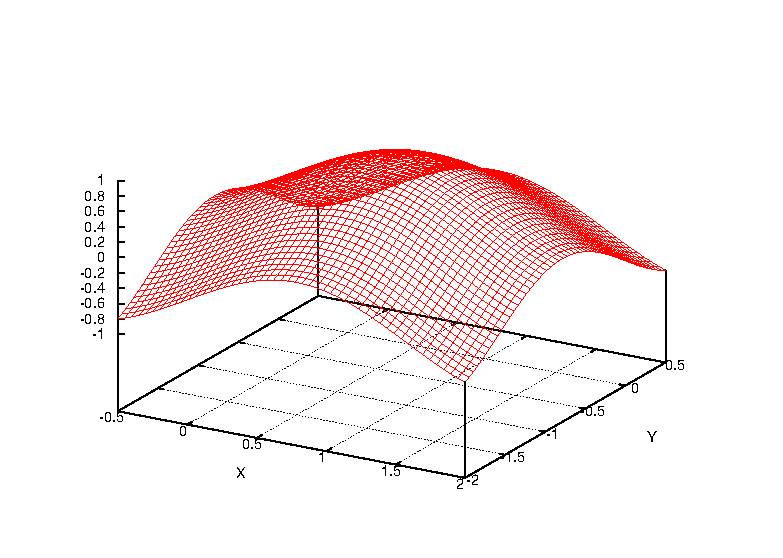
\includegraphics[scale=0.5]{./images/exact.eps}
  \caption{Exact Solution of Poisson's Equation}
  \label{fig:exactPoiss}
\end{figure}

Two simulation runs were performed -- one in serial mode and the other
one in parallel mode using the Message Passing Interface (MPI) with 16
configured nodes. Both runs are configured with $\delta=0.01$ which
yields 251 grid points. \prettyref{fig:approxPoiss} presents both
graphs with the gradient on the surface illustrating the error
\prettyref{eq:error} in the conjugate gradient method compared to the
analytical solution \prettyref{eq:boundaryCond}.

\begin{equation}
  \label{eq:error}
  \epsilon=|u(x,y)-v_{i,j}|
\end{equation}

\begin{figure}[htb]
  \psfrag{X}[B][B][1][0]{x}
  \psfrag{Y}[B][B][1][0]{y}
  \psfrag{ERR}[B][B][1][270]{$\epsilon$}
  \psfrag{PARALLEL}[B][B][1][0]{Parallel}
  \psfrag{SERIAL}[B][B][1][0]{Serial}
  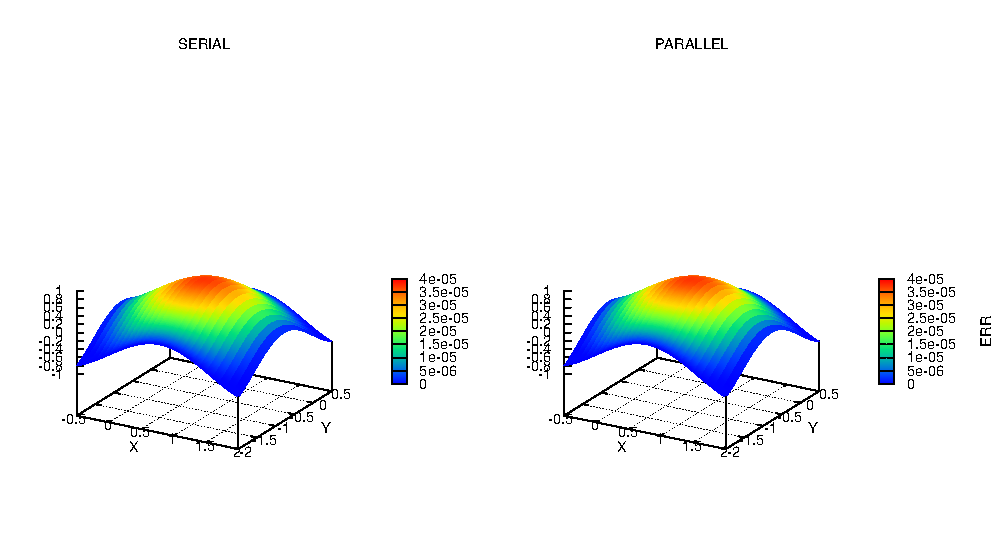
\includegraphics{./images/poiss.eps}
  \caption{Approximate Solution of Poisson's Equation
    $\bigtriangledown^{2}u=-f$}
  \label{fig:approxPoiss}
\end{figure}
    
\end{document}

%%% Local Variables: 
%%% mode: latex
%%% TeX-master: t
%%% End: 
